\chapter{Timeline}

The timeline is displayed at the top of each waveform group and shows the X axis scale for the group. The timeline (and
all accompanying waveform views in the group) may be zoomed by scrolling with the mouse wheel, or panned by dragging
with the left mouse button.

Unlike classical oscilloscope user interfaces, there is \emph{no relationship} between the timeline scale or position
and the duration of the acquisition. It is possible to zoom or scroll beyond the end of the acquisition (displaying
empty background with no signal) or have a deep capture in which nearly all acquired data is offscreen.

Note that the timeline may occasionally show units other than time. For example, an ``eye width" measurement has X axis
units of voltage and Y axis units of time, and a spectrum analyzer channel has X axis units of frequency.


\begin{figure}[h]
\centering
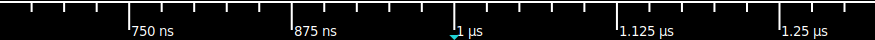
\includegraphics[width=14cm]{images/timeline.png}
\caption{The timeline}
\label{timeline}
\end{figure}

The position of the trigger event is marked by a downward-pointing arrow on the timeline, color coded to match the
channel selected as the primary trigger source. The trigger arrow cannot be interacted with currently, but in the future
(scopehal-apps:173) it will be draggable to adjust the trigger position.

Double-clicking on the timeline brings up the timebase properties dialog (Fig. \ref{timebase-properties}), which allows
the sample rate and memory depth to be configured. If multiple instruments are connected, a separate tab appears in the
dialog for each instrument.

\begin{figure}[h]
\centering
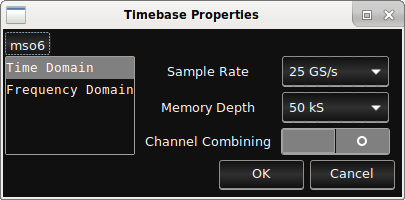
\includegraphics[width=9cm]{images/timebase-properties.png}
\caption{Timebase properties (time domain)}
\label{timebase-properties}
\end{figure}

If the instrument is a spectrum analyzer, or has frequency-domain analysis capability (such as the Tektronix MSO5 and
MSO6 oscilloscopes), the timebase properties dialog will have a second page (Fig. \ref{timebase-properties-freq}) for
setting the span and resolution bandwidth for frequency-domain channels. Center frequency is often a per-channel
adjustment on multichannel instruments, so it is configured from the channel properties dialog rather than timebase
properties.

\begin{figure}[h]
\centering
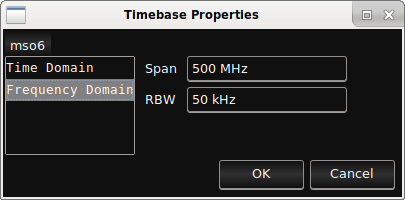
\includegraphics[width=9cm]{images/timebase-properties-freq.png}
\caption{Timebase properties (frequency domain)}
\label{timebase-properties-freq}
\end{figure}
